\documentclass[]{beamer}
\usepackage{graphicx}

\title{Auto-encoders voor compressie}
\author{Josse Van Delm}
\usetheme{Luebeck}
\addtobeamertemplate{navigation symbols}{}{%
    \usebeamerfont{footline}%
    \usebeamercolor[fg]{footline}%
    \hspace{1em}%
    \insertframenumber/\inserttotalframenumber
}

\begin{document}

\begin{frame}
	\frametitle{compressie-algoritme ontwerpen?}
	\pause
	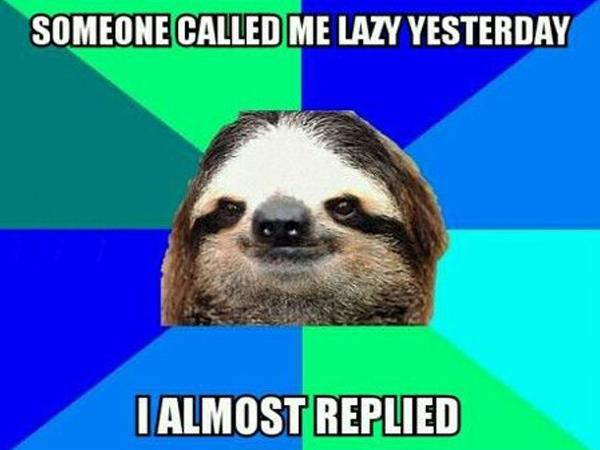
\includegraphics[height =0.85 \textheight]{lazy.jpg}
\end{frame}

\begin{frame}
	\maketitle
\end{frame}

\begin{frame}
	\frametitle{Overzicht}
	\begin{itemize} \pause
		\item Introductie \pause
		\item Auto-encoder \pause
		\item Training \pause
		\item Resultaten 
	\end{itemize}
\end{frame}

\section{Introductie}
\begin{frame}
	\frametitle{Als het bij beeldverwerking lukt,....}
	\begin{itemize} \pause
		\item klassieke beeldverwerking \pause
		\item machine learning - shallow learning \pause
		\item neural networks - deep learning  \pause
	\end{itemize}
	\emph{...werkt het dan ook bij compressie?} \pause

	\begin{center}
		\textbf{\large{Kunnen we iets maken dat beter presteert dan jpeg?}}
	\end{center}
\end{frame}

\section{Auto-encoder}
\begin{frame}
	\frametitle{Een auto-encoder doet aan unsupervised learning}
	\centering
	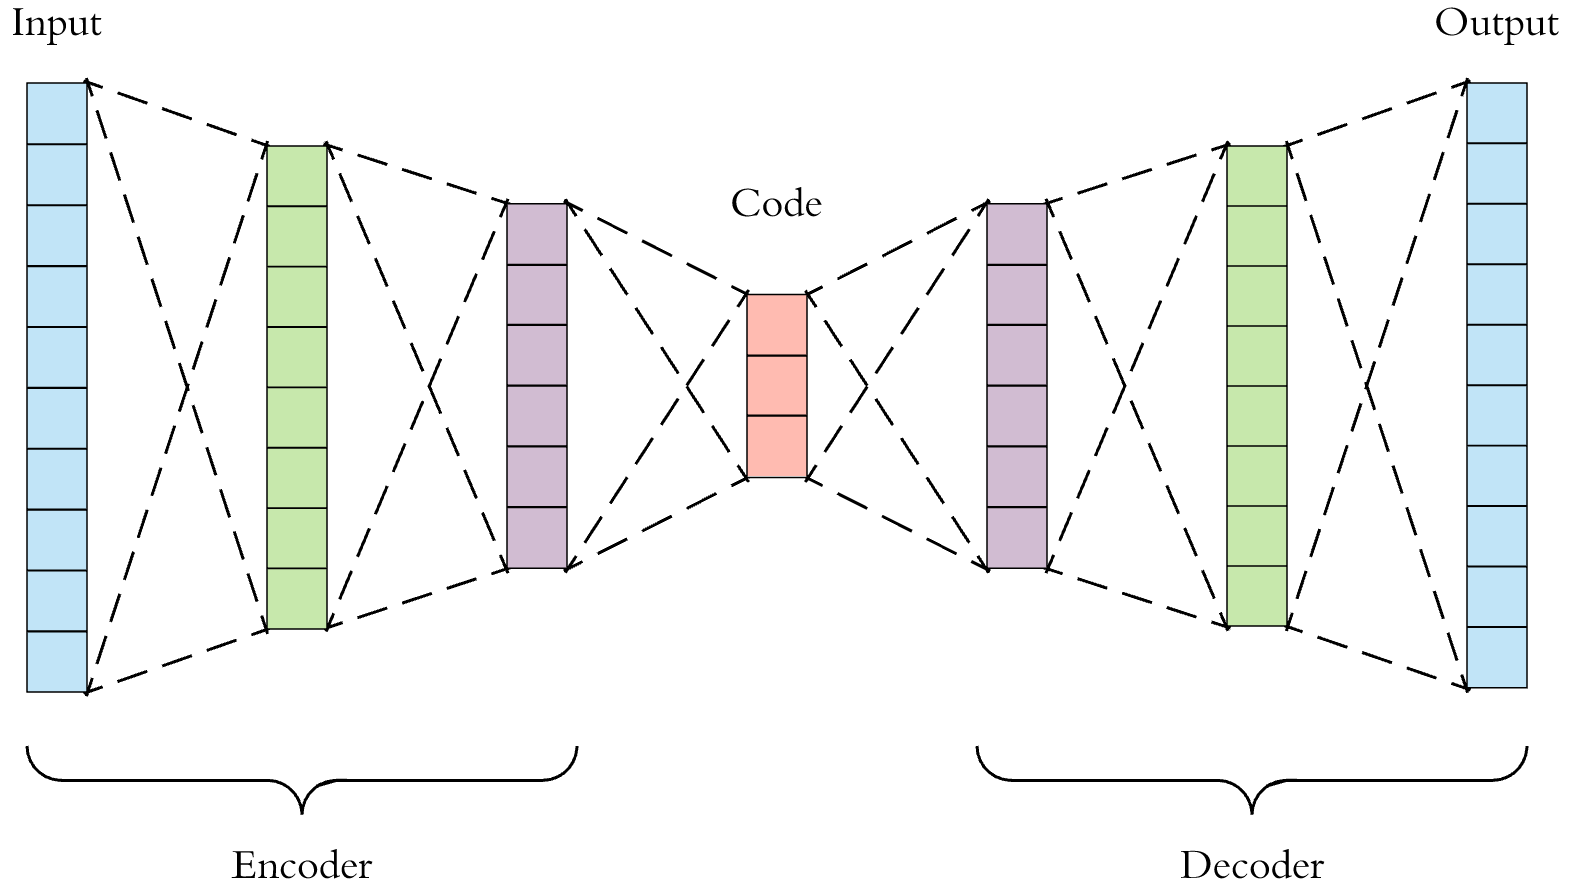
\includegraphics[width = 0.8\textwidth,height = 0.6 \textheight]{autoencoder.png}

	\footnotesize{Bron: https://towardsdatascience.com/applied-deep-learning-part-3-autoencoders-1c083af4d798}
\end{frame}

\begin{frame}
	\frametitle{We gebruiken de latent space als compressiedata}
	\centering
	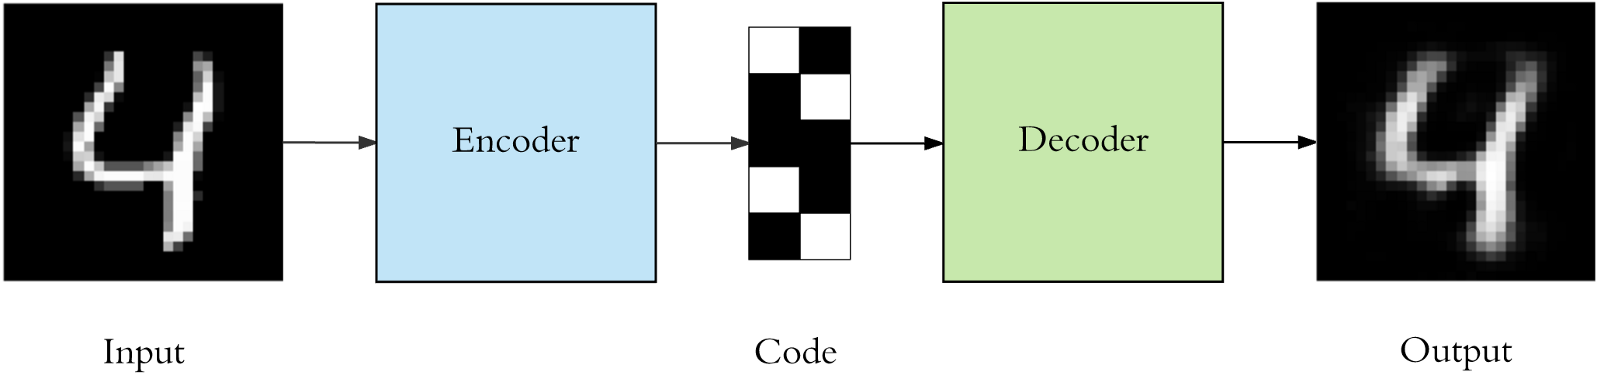
\includegraphics[width = \textwidth]{blockdiagram.png}
	\footnotesize{Bron: https://towardsdatascience.com/applied-deep-learning-part-3-autoencoders-1c083af4d798}
\end{frame}

\begin{frame}
	\frametitle{We gebruiken de latent space als compressiedata}
	Het idee: \pause
	\begin{itemize}
		\item Train auto-encoder \pause
		\item Splits auto-encoder op \pause
		\item Encoder: afbeelding $\rightarrow$ latent space \pause
		\item Decoder: latent space $\rightarrow$ afbeelding
	\end{itemize}
\end{frame}

\section{Training}

\begin{frame}
	\frametitle{De cpu is te traag, en installatie is vervelend}
	We gebruikten:\pause
	\begin{itemize}
		\item Keras deep learning framework frontend \pause
		\item Tensorflow backend \pause
		\item Jupyter Notebook (interactive python shell) \pause
		\item Matplotlib (MATLAB-style plotting) \pause
		\item Docker Container \pause
	\end{itemize}
	implementatie op github!
\end{frame}

\begin{frame}
	\frametitle{Ons netwerk is erg simpel}
	Het bestaat uit:\pause
	\begin{itemize}
		\item \emph{Input}       : afbeelding = $ 28 \cdot 28 \cdot 1 = 784$ waarden (grijswaarden) \pause
		\item \emph{Encoder}     : 3 $\cdot$ (Convolution + Max pooling) \pause
		\item \emph{Latent space}: tensor = $4 \cdot 4 \cdot 8 = 128$ waarden \pause
		\item \emph{Decoder}     : 3 $\cdot$ (Convolution + Upsampling) \pause
		\item \emph{Output}      : afbeelding = $ 28 \cdot 28 \cdot 1 = 784$ waarden (grijswaarden) \pause
	\end{itemize}
	\emph{We mikken dus op een compressieratio van: \textbf{6,125:1}}
\end{frame}

\begin{frame}
	\frametitle{Ons doel is het verkleinen van de loss}
	We werken met de MNIST dataset
	\vspace{10 mm}

	\centering
	
\includegraphics[width = \textwidth]{mnist.png}
\end{frame}

\section{Resultaten}
\begin{frame}
	\frametitle{We kunnen zien dat de loss kleiner wordt}
	\centering
	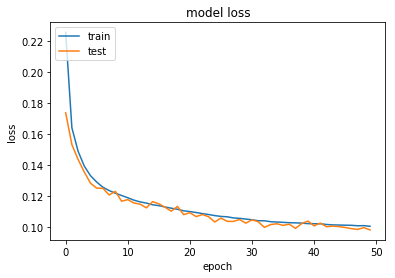
\includegraphics[height = 0.8\textheight]{loss.png}
\end{frame}

\begin{frame}
	\frametitle{De cijfers lijken op elkaar $\rightarrow$ lage loss}
	\centering
	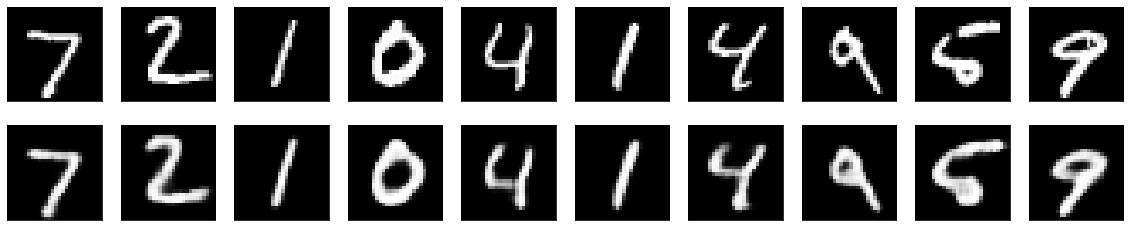
\includegraphics[width = \textwidth]{mnistreconstruction}
\end{frame}

\begin{frame}
	\frametitle{De resultaten vallen een beetje tegen}
	Deze aanpak heeft veel nadelen: \pause
	\begin{itemize}
		\item resultaten erg afhankelijk van trainingsdata \pause
		\item grote netwerken $\rightarrow$ veel computer-resources bij inferentie \pause
		\item Onze aanpak is erg beperkt (28 $\cdot$ 28 grijswaarden) \pause
		\item JPEG haalt gemakkelijk grotere compressieratios! \pause
	\end{itemize}
\end{frame}

\begin{frame}
	\frametitle{Demo!}
	\centering
	Wel,... ongeveer :(
\end{frame}

\begin{frame}
	\centering
	
\includegraphics[height = 0.6\textheight]{jpeg.jpg}
	
	Bedankt voor jullie aandacht! Vragen?
\end{frame}

\end{document}
